 \section{Selector ODP}\begin{description}
\item [CLASSIFICATION:] Good Practice.

\item [MOTIVATION:] Selectors are widely used in the biomedical domain, especially in the realm of anatomy. A selector is a modifier that can be used to select between identical entities, e.g. right and left hand. Selectors are usually associated with simmetry (left-right,anterior-posterior,lateral-medial) and sometimes hard coded in ontologies, that is, for example left hand and right hand are introduced as subclasses of hand, which adds an unecessary amount of classes. This ODP avoids such proliferation of classes.

\item [AIM:] To recreate selectors, that is refining entities that can be used to choose between to alternatives: for example, right or left hand.

\item [STRUCTURE:] See Figure \ref{odp:Selector_abstract}.
\begin{figure}[]\centering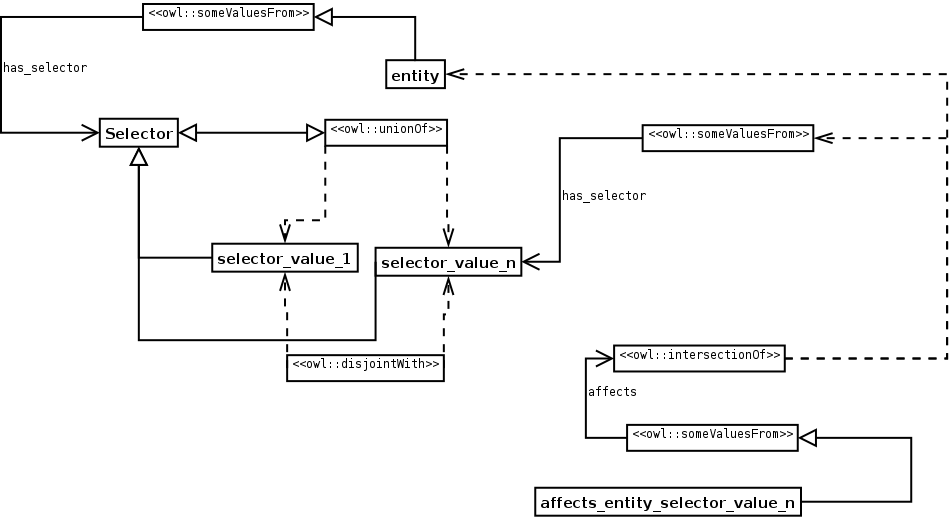
\includegraphics[width=\textwidth]{Catalogue/Selector_abstract}\caption{\label{odp:Selector_abstract} Abstract structure of the Selector ODP.}\end{figure}

\item [SAMPLE:] See Figure \ref{odp:Selector_instance}.
\begin{figure}[]\centering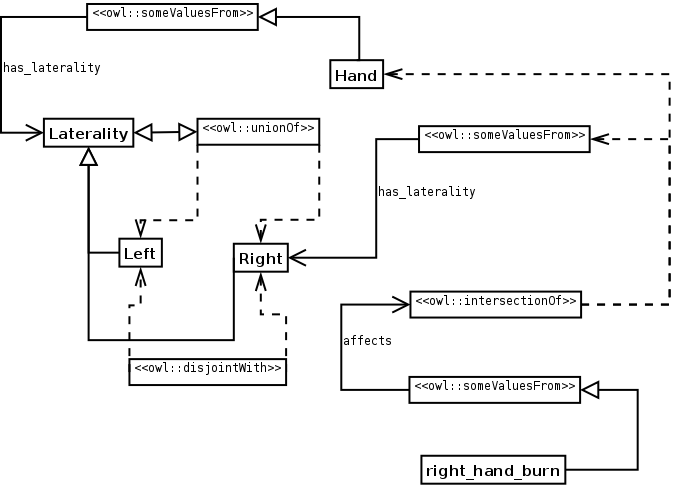
\includegraphics[width=\textwidth]{Catalogue/Selector_instance}\caption{\label{odp:Selector_instance} Sample structure of the Selector ODP.}\end{figure}

\item [ELEMENTS:] The main element is the selector class, be it Laterality (covered by Left and Right), AnteriorPosteriorSelector (covered by Anterior and Posterior), etc. A functional object property, e.g. HasLaterality, is used to add a selector to the classes of the domain hierarchy (e.g. hand can be left or right).

\item [IMPLEMENTATION:] Usually this ODP is implemented in already existing ontologies where selectors are implicit. For example, in the FMA ontology, the class Hand has the subclasses LeftHand and RightHand. Using this ODP, the classes LeftHand and RightHand can be deleted, and the class Hand is linked to the class Laterality via an existential restriction on the HasLaterality property.

\item [RESULT:] The original ontology is considerably reduced in size. If we want to refer the original entities, we can do it by reusing the HasSelector property. For example, if we want to define a burn on the right hand, we can use the following expression: [Burn and Affects some (Hand and HasLaterality some Right)].

\item [SIDE EFFECTS:] Depending on the selection procedure, information could be lost when deleting the subclasses (e.g. RightHand), as they can have further subclasses or interesting axioms.

\item [ADDITIONAL INFORMATION:] See also Entity-Feature-Value, Entity-Property-Value and Entity-Quality.

\item [REFERENCES: ] ~\begin{itemize}
\item Alan Rector (Personal Communication).
\item Eleni Mikroyannidi. Abstracting and generalising a large anatomy ontology. MSc Dissertation, Computer Science, Uni. of Manchester. 2008.\end{itemize}
\item [URL: ] \url{http://www.gong.manchester.ac.uk/odp/owl/Good_Practice_ODP/Selector.owl} \end{description}